%======================================================================
\section{Optimización multiobjetivo en una página}
%======================================================================

\subsection{Dominancia y frente de Pareto}

Escribimos los objetivos como cantidades a \emph{minimizar}: por ejemplo
$f = (-P,\,-\eta,\,\Delta P)$ (maximizar potencia y eficiencia, minimizar fluctuaciones) o
$f = (-P,\,\Delta P,\,\Sigma)$. Un motor $A$ \textbf{domina} a $B$ si es al menos igual de bueno en
todos los objetivos y estrictamente mejor en alguno. Los motores que nadie domina forman el
\textbf{conjunto de Pareto}; sus valores de $f$, el \textbf{frente de Pareto}. Con tres objetivos
el frente es (genéricamente) una superficie.

En el Otto, las variables de decisión son cuatro: $\omega_h\in[0.1,10]$, $r = \omega_c/\omega_h \in
[T_c/T_h, 1]$, $\log_{10}\tau_h$ y $\log_{10}\tau_c \in [-2, 1]$.

\subsection{Figuras de mérito lineales}

En física es habitual condensar los objetivos en un solo número:
\begin{equation}
F = a\,\frac{P}{\Pmax} + b\,\eta - c\,\frac{\Delta P}{\Delta P_0}
\qquad\text{o}\qquad
F = a\,\frac{P}{\Pmax} - b\,\frac{\Delta P}{\Delta P_0} - c\,\frac{\Sigma}{\Sigma_0},
\end{equation}
con pesos $a,b,c\ge0$. La segunda es la de Erdman \emph{et al.} (2023). La ``función ecológica''
$P - T_c\Sigma$ de la termodinámica de tiempo finito es otro ejemplo lineal. Barriendo los pesos se
obtiene una familia de motores óptimos que se espera cubra el frente.

\subsection{Puntos soportados}

\begin{definicion}
Un punto $p$ del frente $\mathcal{F}$ es \textbf{soportado} si existen pesos $w\ge0$,
$\sum_i w_i = 1$, tales que $p$ minimiza $w\cdot f$ sobre todo $\mathcal{F}$.
\end{definicion}

Geométricamente: existe un plano (con normal de componentes no negativas) que toca el frente en $p$
y deja todo el frente de un lado. Todo maximizador de una figura de mérito lineal con pesos no
negativos es soportado, y viceversa. Entonces:

\begin{idea}
El conjunto de motores que una figura de mérito lineal puede encontrar, \emph{para cualquier
elección de pesos}, es exactamente el conjunto de puntos soportados del frente. Si el frente es
convexo, son todos. Si tiene partes no convexas, esas partes son invisibles para la suma ponderada
(Fig.~\ref{fig:legendre}, izquierda).
\end{idea}

Esto es un resultado clásico de optimización multicriterio (Das y Dennis 1997; Ehrgott 2005). Lo
nuevo del proyecto es preguntar cómo depende de \emph{qué variables termodinámicas} se usan.

\begin{figure}[h]
\centering
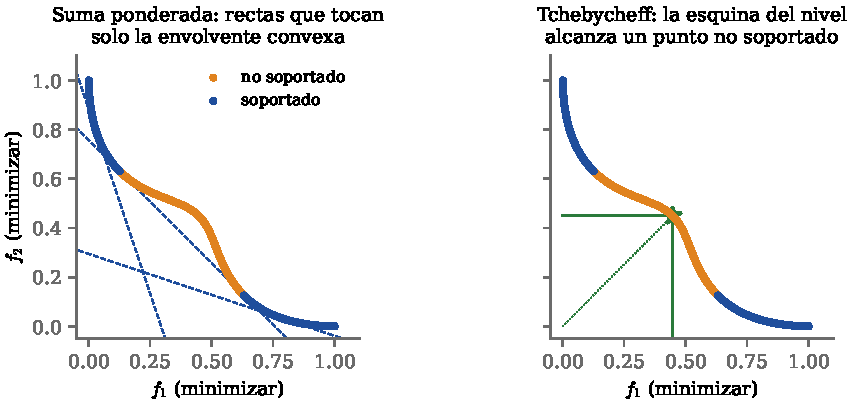
\includegraphics[width=0.95\linewidth]{figs/legendre.pdf}
\caption{Un frente de dos objetivos con una ``abolladura''. Izquierda: cada suma ponderada es una
recta que se desliza hasta tocar el frente; solo toca la envolvente convexa (azul), nunca la parte
naranja. Derecha: la escalarización de Tchebycheff, $\max_i w_i(f_i - z_i)$, tiene curvas de nivel
en forma de esquina; con los pesos adecuados, la esquina alcanza cualquier punto de Pareto,
incluidos los no soportados.}
\label{fig:legendre}
\end{figure}

\subsection{Dos propiedades útiles}

\begin{enumerate}
\item \textbf{Invariancia de escala.} Si cada objetivo se reescala como $f_i \to \alpha_i f_i +
  \beta_i$ con $\alpha_i > 0$, los puntos soportados no cambian (los pesos se reabsorben,
  ejercicio~\ref{ej:escala}). Por eso normalizar por $\Pmax$ o $\Delta P(\Pmax)$ no altera nada.
\item \textbf{Tchebycheff lo alcanza todo.} Con punto ideal $z$ y pesos
  $w_i \propto 1/(f_i(p) - z_i)$, cualquier punto de Pareto $p$ minimiza $\max_i w_i(f_i - z_i)$
  (ejercicio~\ref{ej:tcheby}). Por eso MOEA/D con Tchebycheff no sufre el problema.
\end{enumerate}

\subsection{El test numérico de soporte}

Con un frente muestreado (miles de puntos), ¿cómo saber si un punto es soportado? Se resuelve el
programa lineal
\begin{equation}
s^*(p) = \min_{w\ge0,\ \sum w_i = 1}\ \max_{q\in\mathcal{F}}\ w\cdot\bigl(f(p) - f(q)\bigr).
\label{eq:gap}
\end{equation}
Si $s^* = 0$, existe un peso para el que $p$ es el mejor: soportado. Si $s^* > 0$, para todo peso
hay algún $q$ mejor que $p$, y $s^*$ mide cuánto le falta (en unidades normalizadas). Se escribe como
LP introduciendo la variable $s$: minimizar $s$ sujeto a $w\cdot(f(p)-f(q)) \le s$ para todo $q$.
Usamos tolerancia $s^* > 10^{-3}$ para declarar ``no soportado''. Es \code{support\_gap} en
\code{otto/analysis.py}.

%======================================================================
\section{El resultado central: silla contra tazón}
\label{sec:prop}
%======================================================================

\subsection{Enunciado}

\begin{proposicion}
\label{prop}
Supongamos que
\begin{itemize}
\item[\textbf{(H1)}] el frente de Pareto satura la TUR, $\Delta P = g(P,\eta)$ con $g$ dada por la
  ec.~\eqref{eq:g}, y
\item[\textbf{(H2)}] el frente es una región \emph{bidimensional} de esa superficie: potencia y
  eficiencia se pueden variar de forma independiente (el dominio $D$ de $(P,\eta)$ tiene interior).
\end{itemize}
Entonces:
\begin{enumerate}
\item[(i)] en las variables $f = (-P,-\eta,\Delta P)$, \textbf{ningún punto interior del frente es
  soportado};
\item[(ii)] en las variables $f = (-P,\Delta P,\Sigma)$ la misma superficie es la gráfica de
  $h(P,\Sigma) = 2P^2/\Sigma$, que es \textbf{convexa}. Si el dominio en el plano $(P,\Sigma)$ es
  convexo, todo punto es soportado, aunque de forma \textbf{degenerada}: cada suma ponderada que lo
  soporta tiene un segmento entero de óptimos a lo largo de un rayo $P\propto\Sigma$.
\end{enumerate}
\end{proposicion}

\subsection{Demostración de (i): la silla}

Supongamos que un punto interior $(P_0,\eta_0)$ minimiza
$\phi(P,\eta) = -w_1P - w_2\eta + w_3\,g(P,\eta)$.
\begin{itemize}
\item Si $w_3 = 0$, $\phi$ es lineal y no constante; una función lineal no tiene mínimos en el
  interior de un conjunto abierto. Contradicción. Luego $w_3 > 0$.
\item Con $w_3 > 0$, un mínimo interior exige (condición necesaria de segundo orden) que el
  hessiano de $\phi$, que es $w_3\nabla^2 g$, sea semidefinido positivo.
\end{itemize}
Calculemos el hessiano de $g = 2T_c\,\eta P/(\etaC - \eta)$:
\begin{equation}
g_{PP} = 0,\qquad
g_{P\eta} = \frac{2T_c\,\etaC}{(\etaC-\eta)^2},\qquad
g_{\eta\eta} = \frac{4T_c\,\etaC\,P}{(\etaC-\eta)^3},
\end{equation}
\begin{equation}
\det\nabla^2 g = g_{PP}\,g_{\eta\eta} - g_{P\eta}^2 = -\frac{4T_c^2\,\etaC^2}{(\etaC-\eta)^4} < 0 .
\end{equation}
Un determinante negativo significa un autovalor positivo y uno negativo: el hessiano es
\emph{indefinido}. Contradicción. \hfill$\square$

\paragraph{Intuición.} A $\eta$ fija, $\Delta P$ es \emph{proporcional} a $P$: una recta, curvatura
cero. Pero la pendiente de esa recta, $2T_c\eta/(\etaC-\eta)$, crece con $\eta$. Una superficie que
es recta en una dirección y ``se tuerce'' al moverse en la otra es, localmente, como $z = xy$: el
paraboloide hiperbólico, la silla de montar clásica (Fig.~\ref{fig:silla}, izquierda). Un plano no
puede apoyarse en una silla sin cortarla.

\begin{figure}[h]
\centering
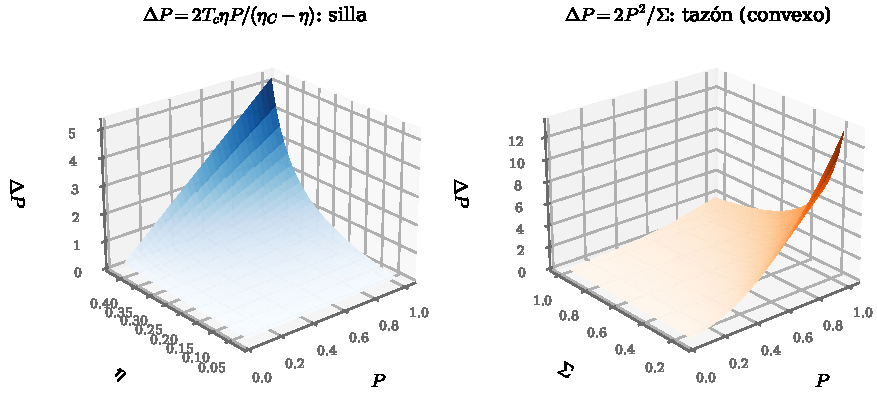
\includegraphics[width=0.95\linewidth]{figs/silla.pdf}
\caption{La misma superficie de saturación de la TUR en dos sistemas de coordenadas. Izquierda:
$(P,\eta,\Delta P)$, una silla (rectas en la dirección de $P$ con pendiente que crece con $\eta$).
Derecha: $(P,\Sigma,\Delta P)$, un tazón convexo, plano a lo largo de los rayos $P\propto\Sigma$.}
\label{fig:silla}
\end{figure}

\subsection{Demostración de (ii): el tazón}

Sustituyendo $\eta = \etaC P/(P+T_c\Sigma)$ (ec.~\ref{eq:sigma}) en $g$:
\[
\frac{2T_c\,\eta}{\etaC-\eta} = \frac{2T_c\cdot\etaC P/(P+T_c\Sigma)}{\etaC T_c\Sigma/(P+T_c\Sigma)}
= \frac{2P}{\Sigma}
\quad\Longrightarrow\quad
\Delta P = \frac{2P^2}{\Sigma}.
\]
(Es simplemente la TUR \eqref{eq:tur} con igualdad.) La función $h(P,\Sigma) = 2P^2/\Sigma$ es la
\emph{perspectiva} de $2P^2$, una construcción que preserva la convexidad (Boyd y Vandenberghe). Su
hessiano,
\begin{equation}
\nabla^2 h = \frac{4}{\Sigma^3}\begin{pmatrix}\Sigma^2 & -P\Sigma\\ -P\Sigma & P^2\end{pmatrix},
\qquad \operatorname{tr} > 0,\quad \det = 0,
\end{equation}
es semidefinido positivo, con dirección nula $(P,\Sigma)$. Para una función convexa, el plano
tangente en cualquier punto queda por debajo de toda la gráfica, así que soporta el punto. Los pesos
correspondientes para $(-P,\Delta P,\Sigma)$ son proporcionales a
$\bigl(\partial_P h,\ 1,\ -\partial_\Sigma h\bigr) = \bigl(4P/\Sigma,\ 1,\ 2P^2/\Sigma^2\bigr)$, todos no
negativos, como debe ser. \hfill$\square$

\subsection{Por qué importan las dos hipótesis}

\begin{itemize}
\item \textbf{Sin (H1)}, la superficie no es la de la ec.~\eqref{eq:g} y no hay razón para la silla.
  Lo veremos en el modelo de control por tramos (sección~\ref{sec:tramos}).
\item \textbf{Sin (H2)}, el frente es una \emph{curva} sobre la silla. Una curva puede estar contenida
  en una silla y aun así ser completamente soportada (piense en una recta trazada sobre $z=xy$). Es
  lo que pasa en respuesta lineal (sección~\ref{sec:lr}).
\end{itemize}
Además, la proposición no dice nada del \emph{borde} del frente: ahí puede haber puntos soportados,
y en la práctica los soportados en $(P,\eta,\Delta P)$ están en partes del borde.

\paragraph{Verificación simbólica.} \code{scripts/geometria.py} calcula estos hessianos con
\texttt{sympy} y aplica el test de soporte a una superficie sintética que satura la TUR: en
$(P,\eta,\Delta P)$ el 85--86\% de los puntos no es soportado (solo bordes); en $(P,\Delta P,\Sigma)$,
0\%.

%======================================================================
\section{La conexión con mecánica estadística}
\label{sec:legendre}
%======================================================================

Esta sección no es necesaria para el resultado, pero es la mejor forma de entenderlo con lo que
sabes del curso.

\subsection{La suma ponderada es una transformada de Legendre}

Maximizar una figura de mérito lineal sobre el frente,
\begin{equation}
F^*(a) = \max_{p\in\mathcal{F}}\ \bigl(a_1 P + a_2\eta - a_3\Delta P\bigr),
\end{equation}
es calcular la \textbf{transformada de Legendre--Fenchel} del frente (su ``función soporte''). Los
pesos son las variables conjugadas. Y la transformada de Legendre tiene una propiedad conocida:
\emph{solo ve la envolvente convexa}. Si transformas dos veces, no recuperas la función original
sino su envolvente convexa.

\subsection{Inequivalencia de ensambles y construcción de Maxwell}

En mecánica estadística pasa exactamente lo mismo al ir del ensamble microcanónico al canónico. La
energía libre es una transformada de Legendre de la entropía:
\begin{equation}
\beta F(\beta) = \min_E\ \bigl(\beta E - S(E)\bigr).
\end{equation}
Si $S(E)$ es cóncava, cada temperatura selecciona una energía y los dos ensambles son
equivalentes. Si $S(E)$ tiene una parte no cóncava (una transición de primer orden, o sistemas con
interacciones de largo alcance), \emph{ninguna temperatura selecciona esas energías}: el ensamble
canónico se las salta y ``rellena'' con la envolvente cóncava. Es la \textbf{construcción de
Maxwell}, y en sistemas de largo alcance se llama \textbf{inequivalencia de ensambles}.

\begin{center}
\begin{tabular}{ll}
\toprule
\textbf{Mecánica estadística} & \textbf{Optimización del motor}\\
\midrule
entropía microcanónica $S(E)$ & frente de Pareto\\
temperatura $\beta$ (variable conjugada) & pesos $(a,b,c)$ de la figura de mérito\\
energía libre $F(\beta)$ (Legendre) & figura de mérito óptima $F^*(a,b,c)$\\
estados que el canónico no selecciona & puntos no soportados\\
construcción de Maxwell & envolvente convexa del frente\\
\bottomrule
\end{tabular}
\end{center}

\begin{idea}[La misma idea, en una frase]
Una figura de mérito lineal es un ``ensamble canónico'' sobre los motores: los pesos hacen de
temperatura. Igual que el ensamble canónico no ve los estados de una región no cóncava de
$S(E)$, la suma ponderada no ve los motores de una región no convexa del frente.
\end{idea}

\subsection{La degeneración en $\Sigma$ es extensividad}

La función $h(P,\Sigma) = 2P^2/\Sigma$ es \textbf{homogénea de grado 1}: $h(\lambda P,\lambda\Sigma) =
\lambda\,h(P,\Sigma)$. Físicamente: dos motores idénticos funcionando en paralelo tienen el doble de
potencia, el doble de producción de entropía y el doble de varianza (si son independientes). Es
\textbf{extensividad}. Una función homogénea de grado 1 es lineal a lo largo de los rayos desde el
origen, y por eso su hessiano tiene un autovalor cero en esa dirección.

Es exactamente lo que pasa con $S(U,V,N)$, también homogénea de grado 1 (relación de Euler): su
hessiano es singular en la dirección $(U,V,N)$. En termodinámica eso no causa problemas; en la suma
ponderada causa \emph{degeneración}: el óptimo no es único a lo largo de cada rayo, y un algoritmo
basado en suma ponderada tiende a amontonar soluciones. Lo veremos en los números (MOEA/D-WS
devuelve solo 68 soluciones distintas de 105).

\subsection{La convexidad depende de las variables}

En el curso se ve que $S(U,V,N)$ es cóncava en sus variables \emph{extensivas naturales}. Escrita
en otras variables (por ejemplo, intensivas) puede dejar de serlo; por eso los potenciales
termodinámicos se definen con transformadas de Legendre y no con cambios de variable arbitrarios.
Nuestro resultado es la versión ``frente de Pareto'' de esa lección: $(P,\Delta P,\Sigma)$ son
cantidades extensivas en el tiempo (tasas que se suman), mientras que $\eta = W/Q_h$ es un
\emph{cociente}, una variable intensiva. Usar un cociente como coordenada rompe la convexidad.

\subsection{Una generalización (derivada para esta guía, por verificar con cuidado)}

La silla no depende de la forma exacta de la TUR. Si el frente es cualquier superficie de la forma
$\Delta P = P\,\varphi(\eta)$ con $\varphi'\neq0$ (fluctuaciones proporcionales a la potencia a
eficiencia fija), entonces
\begin{equation}
\nabla^2(P\varphi) = \begin{pmatrix}0 & \varphi'\\ \varphi' & P\varphi''\end{pmatrix},\qquad
\det = -\varphi'^2 < 0 .
\end{equation}
Siempre es una silla. En variables $(P,\Sigma)$, como $\eta$ depende solo de $t = P/\Sigma$, se tiene
$\Delta P = \Sigma\,\chi(t)$ con $\chi(t) = t\,\varphi(\eta(t))$: la perspectiva de $\chi$, que es
convexa si y solo si $\chi$ lo es. Para la TUR, $\varphi(\eta(t)) = 2t$ y $\chi(t) = 2t^2$. Esto
podría convertir la proposición en un criterio general; es una línea abierta para el paper.

%======================================================================
\section{El límite de respuesta lineal}
\label{sec:lr}
%======================================================================

\subsection{Onsager}

Cerca del equilibrio, los flujos son lineales en las fuerzas termodinámicas:
\begin{equation}
J_1 = L_{11}A_1 + L_{12}A_2,\qquad J_2 = L_{12}A_1 + L_{22}A_2 ,
\end{equation}
con $L$ simétrica (reciprocidad de Onsager) y semidefinida positiva (segunda ley). Para un motor, el
par 2 es el flujo de calor impulsado por la diferencia de temperaturas y el par 1 es el trabajo
contra una fuerza externa. La producción de entropía es $\Sigma = A_1J_1 + A_2J_2$, la potencia
$P = -A_1J_1$ (con $T=1$), la eficiencia relativa a Carnot $\bar\eta = \eta/\etaC = -A_1J_1/(A_2J_2)$,
y la varianza de la potencia (Green--Kubo) $\sigma_P^2 = 2A_1^2L_{11}$.

El acoplamiento se mide con $q = L_{12}/\sqrt{L_{11}L_{22}}\in[-1,1]$; $|q| = 1$ es
\textbf{acoplamiento fuerte} (máquina endorreversible).

\subsection{Todo depende de un solo número}

Almanza-Marrero, Roldán y Manzano (2026) obtienen frentes exactos en este régimen maximizando una suma
ponderada que \emph{incluye} $\eta$. ¿Contradice eso nuestra proposición? No. Fijando los recursos
$A_2 = L_{22} = T = 1$ y definiendo $y = \sqrt{L_{11}}\,A_1$:
\begin{equation}
P = -y(y+q),\qquad \bar\eta = \frac{-y(y+q)}{1+qy},\qquad \Sigma = 1 + 2qy + y^2,\qquad \sigma_P^2 = 2y^2 .
\end{equation}
Las cuatro cantidades dependen solo de $(y,q)$. A $y$ fijo, aumentar $q$ aumenta $P$ y $\bar\eta$ y
disminuye $\Sigma$ (ejercicio~\ref{ej:lr}), así que el frente está en $q = 1$. Con $e = -y\in[0,1]$:
\begin{equation}
P = e(1-e),\qquad \bar\eta = e,\qquad \Sigma = (1-e)^2,\qquad \sigma_P^2 = 2e^2 .
\end{equation}
El frente es una \textbf{curva} de un parámetro, $P = 4\Pmax\,\bar\eta(1-\bar\eta)$, y satura la TUR
exactamente: $\sigma_P^2\Sigma = 2e^2(1-e)^2 = 2P^2$. Cumple (H1) pero no (H2).

Maximizar la figura de mérito sobre $e$ es un problema cuadrático cóncavo cuyo óptimo recorre todo
$[0,1]$ al variar los pesos: la suma ponderada es \textbf{exacta}. \code{scripts/almanza.py} lo
verifica con $2\times10^5$ diseños aleatorios: el 99.95\% del frente tiene $q = 1$, el error contra
la curva analítica es $<2\times10^{-5}$, y no hay ningún punto no soportado.

\begin{figure}[h]
\centering
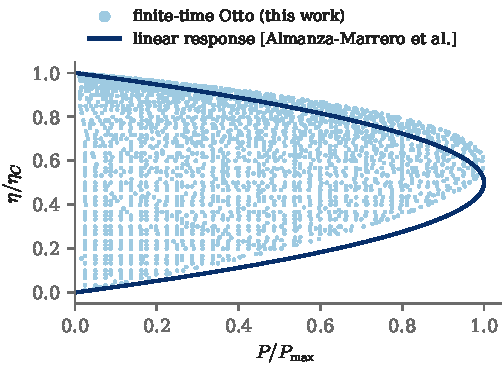
\includegraphics[width=0.55\linewidth]{figs/fig4_linear_response.pdf}
\caption{Frente del Otto en tiempo finito proyectado en $(P,\eta)$ (puntos, bidimensional) y frente
de respuesta lineal (curva). Cada uno normalizado por su propia potencia máxima: la figura compara
dimensiones, no cotas.}
\label{fig:lr}
\end{figure}

\begin{idea}
Cerca del equilibrio hay un solo grado de libertad efectivo: potencia y eficiencia van amarradas.
Lejos del equilibrio se desacoplan, el frente gana una dimensión, y si además satura la TUR, la
suma ponderada con $\eta$ pierde casi todo el interior. El problema aparece justo en el régimen
que motiva optimizar numéricamente.
\end{idea}
